\documentclass[11pt,a4paper]{article}
\usepackage[T1]{fontenc}
\usepackage[utf8]{inputenc}
\usepackage{lmodern}
\usepackage{textcomp}
\usepackage[left=1.8cm,right=1.8cm,top=3.0cm,bottom=2.2cm,headheight=36pt,headsep=12pt]{geometry}
\usepackage{multicol}
\usepackage{xcolor}
\usepackage{fancyhdr}\usepackage{tikz}
\usepackage{graphicx}
\usepackage{array}
\usepackage{amsmath,amssymb}
\usepackage{setspace}
\usepackage{longtable}
\graphicspath{{../}}
\definecolor{ygreen}{RGB}{46,139,87}\definecolor{dgreen}{RGB}{28,90,56}
\renewcommand{\normalsize}{\fontsize{10.9}{13.4}\selectfont}
\renewcommand{\familydefault}{\rmdefault}
\setlength{\parindent}{0pt}
\setlength{\columnsep}{0.8cm}
\setlength{\columnseprule}{0.4pt}
\setlength{\multicolsep}{3pt plus 1pt minus 1pt}
\renewcommand{\textsubscript}[1]{\ensuremath{_{\text{\fontsize{8}{8}\selectfont #1}}}}
\renewcommand{\textsuperscript}[1]{\ensuremath{^{\text{\fontsize{8}{8}\selectfont #1}}}}
\newcommand{\qn}[1]{\textbf{\fontsize{11.5}{13}\selectfont #1}}
\newcommand{\qsep}{\par\vspace{13pt}}
\newcommand{\fwrule}{\par\vspace{5pt}\noindent\rule{\linewidth}{1.4pt}\par\vspace{7pt}}
\newsavebox{\fitb}
\newcommand{\fitbox}[1]{\sbox{\fitb}{#1}\ifdim\wd\fitb>\linewidth\resizebox{\linewidth}{!}{\usebox{\fitb}}\else\usebox{\fitb}\fi}
\newcommand{\diqqat}[1]{\par\smallskip\noindent\textbf{Diqqat!} #1\par\medskip}
\newcommand{\javob}{\par\nopagebreak[4]\smallskip\noindent\textbf{Javob:} \rule[-2pt]{7.5cm}{0.4pt}\par\smallskip\noindent\textbf{Diqqat!} Javobingizni javoblar varaqasiga ko`chirib yozing.\par\medskip}
\pagestyle{fancy}
\fancyhf{}
\renewcommand{\headrulewidth}{1.6pt}\renewcommand{\headrule}{{\color{ygreen}\hrule height 1.6pt width\headwidth}}
\newcommand{\hdrlogo}{
\begin{tikzpicture}[baseline=0pt]\fill[ygreen,rounded corners=3pt] (0,0) rectangle (0.95,0.95);\node[white,font=\fontsize{24}{26}\bfseries\selectfont] at (0.475,0.47){K};\node[anchor=west,font=\fontsize{16}{18}\bfseries\selectfont,text=dgreen] at (1.15,0.66){KIMYO};\node[anchor=west,font=\footnotesize\scshape,text=gray] at (1.15,0.2){Milliy sertifikat\ \ 2026};\end{tikzpicture}}
\newcommand{\hdrpill}[1]{\begin{tikzpicture}[baseline=0pt]\node[fill=ygreen,text=white,rounded corners=8pt,inner xsep=10pt,inner ysep=5pt,font=\fontsize{13}{15}\bfseries\selectfont] at (0,0.475){#1};\end{tikzpicture}}
\fancyhead[L]{\hdrlogo}
\fancyhead[R]{\hdrpill{14-variant}}

\fancyfoot[C]{\thepage}
\fancypagestyle{first}{\fancyhf{}\renewcommand{\headrulewidth}{1.6pt}\renewcommand{\headrule}{{\color{ygreen}\hrule height 1.6pt width\headwidth}}\fancyhead[L]{\hdrlogo}\fancyhead[R]{\hdrpill{14-variant}}\fancyfoot[C]{\thepage}}
\begin{document}
\normalsize
\thispagestyle{first}
\noindent\textit{Davriy jadvaldan foydalanish mumkin.}
\par\smallskip
\begin{multicols}{2}
\noindent\qn{1.} Jadvalda metall plastinkalarning tuz eritmalariga tushirilishidagi kuzatuvlar berilgan (``+'' -- metall ajraladi, reaksiya boradi; ``$-$'' -- reaksiya bormaydi):
\begin{center}
\renewcommand{\arraystretch}{1.15}
\fitbox{\begin{tabular}{|c|c|c|c|}\hline
\textbf{Metall} & \textbf{AgNO\textsubscript{3} eritmasi} & \textbf{FeSO\textsubscript{4} eritmasi} & \textbf{ZnSO\textsubscript{4} eritmasi} \\ \hline
Zn & + & + & $-$ \\ \hline
Ag & $-$ & $-$ & $-$ \\ \hline
Cu & + & $-$ & $-$ \\ \hline
\end{tabular}}
\end{center}
Ushbu metallardan qaysi biri eng faol?

\noindent A)~\textsl{Ag} \hfill B)~\textsl{Cu} \hfill C)~\textsl{Zn} \hfill D)~\textsl{Mg}\par
\qsep
\noindent\qn{2.} ZnSO\textsubscript{4} ning suvli eritmasi inert elektrodlar bilan elektroliz qilinganda qaysi moddalar ajraladi?

\noindent\begin{tabular}{@{}p{0.47\linewidth}@{}p{0.47\linewidth}@{}}
A)~\textsl{Cu va O\textsubscript{2}} & B)~\textsl{Zn, H\textsubscript{2} va O\textsubscript{2}} \\
C)~\textsl{Cu va Cl\textsubscript{2}} & D)~\textsl{Ag va O\textsubscript{2}} \\
\end{tabular}\par
\qsep
\noindent\qn{3.} Na\textsubscript{2}SO\textsubscript{4} ning suvli eritmasi inert elektrodlar bilan elektroliz qilinganda qaysi moddalar ajraladi?

\noindent\begin{tabular}{@{}p{0.47\linewidth}@{}p{0.47\linewidth}@{}}
A)~\textsl{H\textsubscript{2} va O\textsubscript{2}} & B)~\textsl{Cu va O\textsubscript{2}} \\
C)~\textsl{H\textsubscript{2}, Cl\textsubscript{2} va NaOH} & D)~\textsl{Ag va O\textsubscript{2}} \\
\end{tabular}\par
\qsep
\noindent\qn{4.} Alyuminiy (\textit{Z} = 13) atomi elektron konfiguratsiyasida jami nechta juftlashgan elektron bor?

\noindent A)~\textsl{12} \hfill B)~\textsl{13} \hfill C)~\textsl{11} \hfill D)~\textsl{14}\par
\qsep
\noindent\qn{5.} B elementi ikki izotopdan iborat (massa sonlari 10 va 11). O`rtacha nisbiy atom massasi 10,8 bo`lsa, 50 g namunadagi og`ir izotopning \textbf{massasini (g) aniqlang.}

\noindent A)~\textsl{40} \hfill B)~\textsl{40,74} \hfill C)~\textsl{10} \hfill D)~\textsl{44}\par
\qsep
\noindent\qn{6.} 12,3 l SO\textsubscript{2} 27 \textdegree{}C va 1 atm bosimda necha gramm keladi? (R = 0,082 l$\cdot$atm/(mol$\cdot$K))

\noindent A)~\textsl{32} \hfill B)~\textsl{64} \hfill C)~\textsl{16} \hfill D)~\textsl{35,14}\par
\qsep
\noindent\qn{7.} Rasmda Al va Cl atomlari orasida elektron o`tishi sxematik ko`rsatilgan (ion bog` hosil bo`lishi).
\begin{center}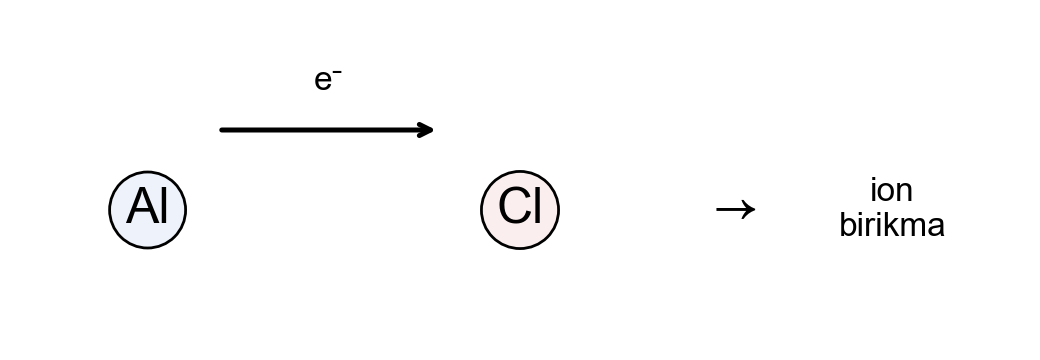
\includegraphics[width=0.86\linewidth]{rasmlar/gen/ib_857918.png}\end{center}
Al atomi qancha elektron berib, qanday zaryadli ionga aylanadi?

\noindent A)~\textsl{3 ta, $-$3} \hfill B)~\textsl{3 ta, +3} \hfill C)~\textsl{4 ta, +4} \hfill D)~\textsl{5 ta, +5}\par
\qsep
\noindent\qn{8.} Reaksiya tezligining harorat koeffitsiyenti $\gamma$ = 3. 30 \textdegree{}C da reaksiya 81 minutda tugasa, 60 \textdegree{}C da necha sekundda tugaydi?

\noindent A)~\textsl{180} \hfill B)~\textsl{131220} \hfill C)~\textsl{540} \hfill D)~\textsl{3}\par
\qsep
\noindent\qn{9.} 1 mol C\textsubscript{3}H\textsubscript{6} va 3 mol HCN aralashmasidagi $\pi$-bog`lar umumiy \textbf{sonini (N\textsubscript{A} birligida) aniqlang.}

\noindent A)~\textsl{7} \hfill B)~\textsl{14} \hfill C)~\textsl{21} \hfill D)~\textsl{1}\par
\qsep
\noindent\qn{10.} Mg va Zn aralashmasi tarkibida Mg ning mol miqdori aralashmadagi umumiy mol miqdorining 1/4 qismini tashkil etadi. Aralashmaning massasi 21,9 g. Aralashmaning zichligi 2,3 g/sm\textsuperscript{3} ga teng. Aralashmadagi Mg ning mol \textbf{ulushini (\%) hisoblang.}

\noindent A)~\textsl{75} \hfill B)~\textsl{10,96} \hfill C)~\textsl{50} \hfill D)~\textsl{25}\par
\qsep
\noindent\qn{11.} 10 ml HCl eritmasi 0,2 mol/l li NaOH eritmasi bilan titrlandi. Titrlash egri chizig`i grafikda berilgan (ekvivalent nuqta 10 ml da).
\begin{center}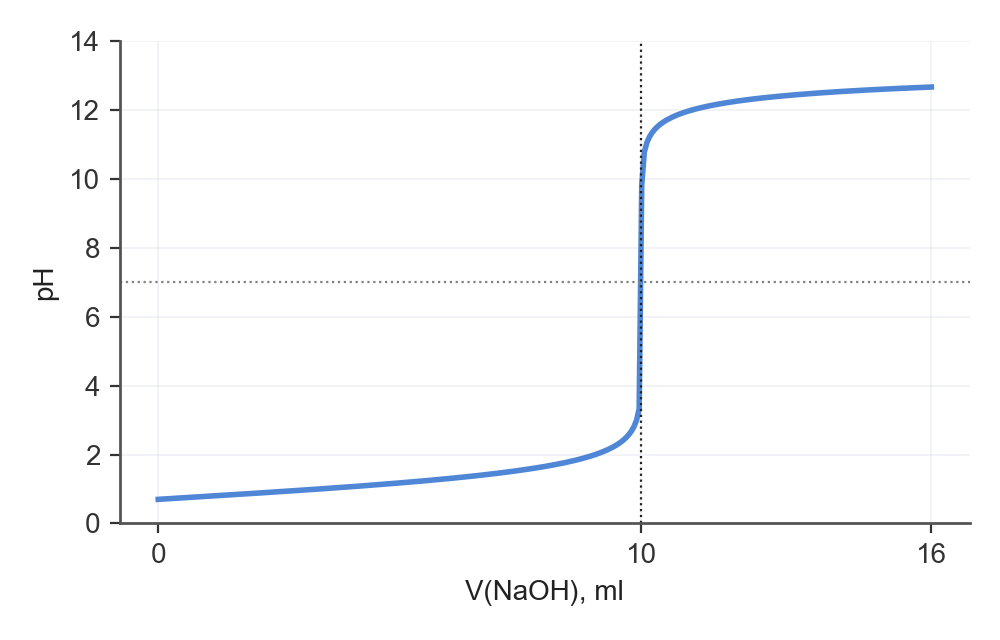
\includegraphics[width=0.86\linewidth]{rasmlar/gen/ti_v14_0.png}\end{center}
Ekvivalent nuqtagacha sarflangan NaOH ning \textbf{massasini (g) hisoblang.}

\noindent A)~\textsl{80} \hfill B)~\textsl{0,16} \hfill C)~\textsl{0,08} \hfill D)~\textsl{0,073}\par
\qsep
\noindent\qn{12.} Laboratoriyada Na\textsubscript{2}CO\textsubscript{3} eritmalari quyidagicha tayyorlangan:
\begin{center}
\renewcommand{\arraystretch}{1.15}
\fitbox{\begin{tabular}{|c|c|c|}\hline
\textbf{Idish} & \textbf{Eritma massasi, g} & \textbf{$\omega$(Na\textsubscript{2}CO\textsubscript{3}), \%} \\ \hline
A & 150 & 5 \\ \hline
B & 100 & 25 \\ \hline
\end{tabular}}
\end{center}
Bu ikki eritma bir idishga quyilib, yangi eritmadagi Na\textsubscript{2}CO\textsubscript{3} ning massa ulushi (\%) qancha bo`ladi?

\noindent A)~\textsl{15} \hfill B)~\textsl{13} \hfill C)~\textsl{30} \hfill D)~\textsl{17}\par
\qsep
\noindent\qn{13.} Na\textsubscript{2}CO\textsubscript{3} va CaCO\textsubscript{3} aralashmasi tarkibida Na\textsubscript{2}CO\textsubscript{3} ning mol miqdori aralashmadagi umumiy mol miqdorining 5/7 qismini tashkil etadi. Aralashmaning massasi 73 g. Aralashmaning zichligi 2,8 g/sm\textsuperscript{3} ga teng. Aralashmadagi Na\textsubscript{2}CO\textsubscript{3} ning \textbf{massasini (g) toping.}

\noindent A)~\textsl{20} \hfill B)~\textsl{106} \hfill C)~\textsl{36,5} \hfill D)~\textsl{53}\par
\qsep
\noindent\qn{14.} Quyidagi jarayonlar qanday kuzatuvlar bilan boradi? To`g`ri ta'riflangan \textbf{jarayonlarni belgilang.} 1) FeCl\textsubscript{3} eritmasiga avval NaOH, so`ng mo`l HCl eritmasi qo`shilganda: qo`ng`ir-qizil cho`kma tushadi, keyin cho`kma erimasdan qoladi; 2) ohakli suvga avval oz, so`ng mo`l CO\textsubscript{2} yuborilganda: eritma loyqalanadi, keyin loyqa yanada quyuqlashadi; 3) AlCl\textsubscript{3} eritmasiga avval oz, so`ng mo`l NaOH eritmasi qo`shilganda: oq cho`kma tushadi, keyin cho`kma erimasdan qoladi; 4) AgNO\textsubscript{3} eritmasiga avval NaCl, so`ng mo`l ammiak eritmasi qo`shilganda: oq tvorogsimon cho`kma tushadi, keyin cho`kma erib ketadi

\noindent A)~\textsl{1, 4} \hfill B)~\textsl{2, 4} \hfill C)~\textsl{2, 3} \hfill D)~\textsl{4}\par
\qsep
\noindent\qn{15.} D-metallar va ularning birikmalari haqida qaysi fikrlar to`g`ri? 1) Mis nam havoda (CuOH)\textsubscript{2}CO\textsubscript{3} qoplamasi bilan qoplanadi; 2) Fe(OH)\textsubscript{2} havoda qo`ng`ir rangga o`tadi; 3) Rux eritmada Fe\textsuperscript{2+} ni siqib chiqara olmaydi; 4) Temir sovuq konsentrlangan HNO\textsubscript{3} da passivlanadi

\noindent A)~\textsl{1, 4} \hfill B)~\textsl{3, 4} \hfill C)~\textsl{1, 3, 4} \hfill D)~\textsl{1, 2, 4}\par
\qsep
\noindent\qn{16.} Qaysi juftliklar o`zaro reaksiyaga kirishmaydi? 1) Fe va HNO\textsubscript{3}(sovuq kons.); 2) ZnO va HCl; 3) Cu va HCl; 4) SiO\textsubscript{2} va H\textsubscript{2}O

\noindent A)~\textsl{1, 2, 3} \hfill B)~\textsl{2, 3, 4} \hfill C)~\textsl{1, 3, 4} \hfill D)~\textsl{1, 2}\par
\qsep
\noindent\qn{17.} 6,9 g natriy suvda eritildi, hosil bo`lgan eritmadan 0,2 mol CO\textsubscript{2} o`tkazildi. Hosil bo`lgan natriy gidrokarbonat \textbf{massasini (g) aniqlang.}

\noindent A)~\textsl{8,4} \hfill B)~\textsl{10,6} \hfill C)~\textsl{16,8} \hfill D)~\textsl{25,2}\par
\qsep
\noindent\qn{18.} CaCO\textsubscript{3} va BaCO\textsubscript{3} aralashmasi (98,8 g) mo`l xlorid kislota bilan ta'sirlashganda 13,44 l (n.sh.) gaz ajraldi. Sarflangan HCl \textbf{massasini (g) hisoblang.}

\noindent A)~\textsl{21,9} \hfill B)~\textsl{87,6} \hfill C)~\textsl{14,6} \hfill D)~\textsl{43,8}\par
\qsep
\noindent\qn{19.} 34,2 g Al\textsubscript{2}(SO\textsubscript{4})\textsubscript{3} eritmasiga mo`l Na\textsubscript{2}S eritmasi qo`shildi (qo`shma gidroliz). Ajralgan gaz \textbf{hajmini (l, n.sh.) hisoblang.}

\noindent A)~\textsl{4,48} \hfill B)~\textsl{13,44} \hfill C)~\textsl{2,24} \hfill D)~\textsl{6,72}\par
\qsep
\noindent\qn{20.} Aldegid va ketonlar haqida qaysi fikrlar to`g`ri? 1) Aldegidlar qaytarilganda ikkilamchi spirt hosil bo`ladi; 2) Ketonlar kuchsiz oksidlovchilar bilan oksidlanmaydi; 3) Sirka aldegid Kucherov reaksiyasi bilan olinadi; 4) Aseton suvda erimaydi

\noindent A)~\textsl{2, 3} \hfill B)~\textsl{2, 4} \hfill C)~\textsl{2, 3, 4} \hfill D)~\textsl{1, 2, 3}\par
\qsep
\noindent\qn{21.} Probirkalardagi organik moddalar: fenol, etanol, glitserin ni alohida probirkalarda ajratish uchun qaysi reagent(lar) yetarli? 1) Na metali; 2) Cu(OH)\textsubscript{2} (sovuqda) va FeCl\textsubscript{3}; 3) Cu(OH)\textsubscript{2} (qizdirilganda) va Na metali; 4) Na metali va FeCl\textsubscript{3}

\noindent A)~\textsl{1, 3} \hfill B)~\textsl{4} \hfill C)~\textsl{2} \hfill D)~\textsl{1}\par
\qsep
\noindent\qn{22.} Yuqori molekulyar birikmalar haqida qaysi fikrlar to`g`ri? 1) Teflon --- polivinilxlorid; 2) Tabiiy kauchuk -- sis-1,4-poliizopren; 3) Kapron poliamid tola; 4) Polietilen polimerlanish reaksiyasi bilan olinadi

\noindent A)~\textsl{2, 4} \hfill B)~\textsl{2, 3} \hfill C)~\textsl{2, 3, 4} \hfill D)~\textsl{1, 2}\par
\qsep
\noindent\qn{23.} Alkanning monobromlanishidan hosil bo`lgan galogenli hosilada brom massa ulushi 58,4\% ga teng. Dastlabki alkan molekulasidagi uglerod atomlari \textbf{sonini toping.}

\noindent A)~\textsl{5} \hfill B)~\textsl{3} \hfill C)~\textsl{4} \hfill D)~\textsl{6}\par
\qsep
\noindent\qn{24.} Metilformiat va etilatsetat aralashmasi (32,4 g) mo`l NaOH eritmasi bilan to`liq gidrolizlandi. Aralashmaning mol miqdori 0,4 mol. Hosil bo`lgan spirtlar \textbf{massasini (g) aniqlang.}

\noindent A)~\textsl{34} \hfill B)~\textsl{15,4} \hfill C)~\textsl{15,6} \hfill D)~\textsl{17}\par
\qsep
\noindent\qn{25.} 360 g glukoza spirtli bijg`ishga uchradi (unum 75\%). Ajralgan gaz mo`l ohakli suvdan o`tkazilganda necha gramm cho`kma hosil bo`ladi?

\noindent A)~\textsl{300} \hfill B)~\textsl{400} \hfill C)~\textsl{150} \hfill D)~\textsl{600}\par
\qsep
\noindent\qn{26.} 810 g kraxmal gidrolizlanib (unum 75\%) glukoza olindi, glukoza esa spirtli bijg`ishga uchradi (unum 80\%). Hosil bo`lgan etanol \textbf{massasini (g) toping.}

\noindent A)~\textsl{138} \hfill B)~\textsl{276} \hfill C)~\textsl{552} \hfill D)~\textsl{345}\par
\qsep
\noindent\qn{27.} 112 l (n.sh.) C\textsubscript{2}H\textsubscript{4} dan quyidagi sxema bo`yicha 38,4 g sirka kislota olindi: C\textsubscript{2}H\textsubscript{4} $\to$ C\textsubscript{2}H\textsubscript{5}OH $\to$ CH\textsubscript{3}CHO $\to$ CH\textsubscript{3}COOH. Dastlabki 2 bosqichning unumi ketma-ket 80\%, 40\% ga teng. Barcha reaksiyalar 1,5 atm bosimda olib borildi. Oxirgi bosqichning \textbf{unumini (\%) aniqlang.}

\noindent A)~\textsl{20} \hfill B)~\textsl{40} \hfill C)~\textsl{60} \hfill D)~\textsl{32}\par
\qsep
\noindent\qn{28.} 368 g C\textsubscript{6}H\textsubscript{5}CH\textsubscript{3} dan quyidagi sxema bo`yicha etilbenzoat olindi: C\textsubscript{6}H\textsubscript{5}CH\textsubscript{3} $\to$ C\textsubscript{6}H\textsubscript{5}COOH $\to$ C\textsubscript{6}H\textsubscript{5}COOC\textsubscript{2}H\textsubscript{5}. Bosqichlarning unumi ketma-ket 75\%, 80\% ni tashkil qiladi. Barcha reaksiyalar 1 atm bosimda olib borildi. Olingan etilbenzoat \textbf{massasini (g) aniqlang.}

\noindent A)~\textsl{720} \hfill B)~\textsl{360} \hfill C)~\textsl{180} \hfill D)~\textsl{450}\par
\qsep
\noindent\qn{29.} 171 g C\textsubscript{12}H\textsubscript{22}O\textsubscript{11} dan quyidagi sxema bo`yicha etanol olindi: C\textsubscript{12}H\textsubscript{22}O\textsubscript{11} $\to$ C\textsubscript{6}H\textsubscript{12}O\textsubscript{6} (glyukoza va fruktoza) $\to$ C\textsubscript{2}H\textsubscript{5}OH. Bosqichlarning unumi ketma-ket 50\%, 60\% ni tashkil qiladi. Barcha reaksiyalar 2 atm bosimda olib borildi. Olingan etanol \textbf{massasini (g) aniqlang.}

\noindent A)~\textsl{55,2} \hfill B)~\textsl{27,6} \hfill C)~\textsl{13,8} \hfill D)~\textsl{46}\par
\qsep
\noindent\qn{30.} Sirka aldegid va aseton eritmalarini (moddalarini) bir-biridan qaysi reagent yordamida farqlash mumkin?

\noindent\begin{tabular}{@{}p{0.47\linewidth}@{}p{0.47\linewidth}@{}}
A)~\textsl{lakmus} & B)~\textsl{temir(III) xlorid} \\
C)~\textsl{ammiakli kumush oksid} & D)~\textsl{natriy metali} \\
\end{tabular}\par
\qsep
\noindent\qn{31.} Eritmaga NaOH qo`shilganda havorang cho`kma (Cu(OH)\textsubscript{2}) kuzatildi. Eritmada qaysi ion bor?

\noindent A)~\textsl{Ag\textsuperscript{+}} \hfill B)~\textsl{Br\textsuperscript{$-$}} \hfill C)~\textsl{Cu\textsuperscript{2+}} \hfill D)~\textsl{SO\textsubscript{4}\textsuperscript{2$-$}}\par
\qsep
\noindent\qn{32.} Rasmdagi asbobda 10 g CaCO\textsubscript{3} ga HCl ta'sir ettirildi. Ajralgan CO\textsubscript{2} \textbf{hajmini (l, n.sh.) aniqlang.}
\begin{center}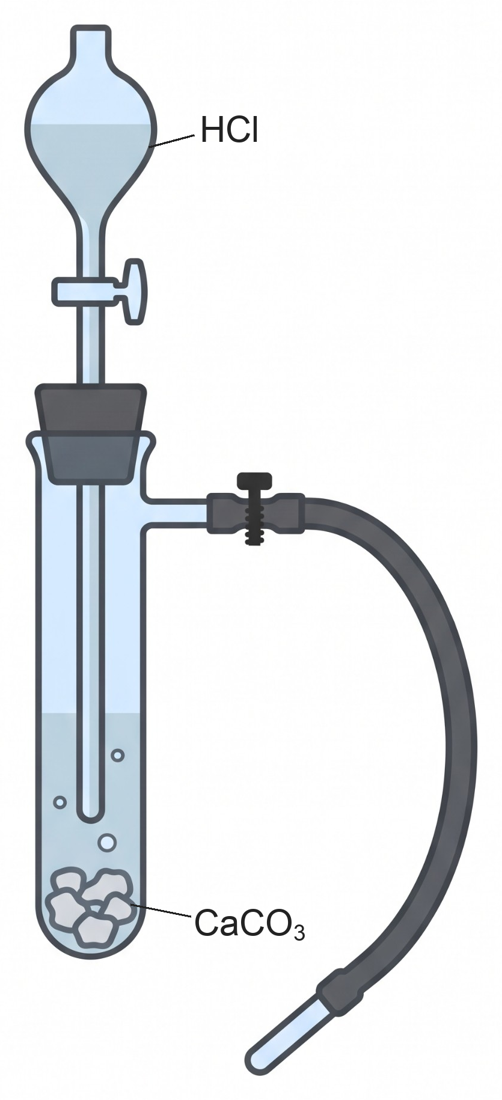
\includegraphics[width=0.86\linewidth]{rasmlar/darslik/d_co2.png}\end{center}

\noindent\begin{tabular}{@{}p{0.47\linewidth}@{}p{0.47\linewidth}@{}}
A)~\textsl{4,48} & B)~\textsl{1,12} \\
C)~\textsl{0,23} & D)~\textsl{2,24   ---} \\
\end{tabular}\par
\qsep
\end{multicols}
\medskip
\noindent\setlength{\fboxsep}{0pt}\fbox{\begin{tabular}{p{0.74\linewidth}|p{0.2\linewidth}}
\parbox[t]{0.72\linewidth}{\vspace{3pt}\textbf{Topshiriqlar (33--35) va javob variant (A--F)larini o`zaro to`g`ri moslashtiring.} Rux va temir qotishmasi (17,7 g) mo`l suyultirilgan H\textsubscript{2}SO\textsubscript{4} da eritilganda 6,72 l (n.sh.) gaz ajraldi; hosil bo`lgan eritmaning hajmi 500 ml. Eritmaga mo`l NaOH qo`shilib, cho`kma ajratildi, havoda to`liq oksidlanguncha tutildi va doimiy massagacha kuydirildi.
\vspace{3pt}} & \parbox[t]{0.19\linewidth}{\vspace{3pt}A~\textsl{0,56}\\[3pt]
B~\textsl{24}\\[3pt]
C~\textsl{16}\\[3pt]
D~\textsl{0,4}\\[3pt]
E~\textsl{1,12}\\[3pt]
F~\textsl{0,8}}\\ \hline
\parbox[t]{0.72\linewidth}{\vspace{2pt}\textbf{33. Eritmada FeSO\textsubscript{4} ning molyar konsentratsiyasini (mol/l) aniqlang.}\vspace{2pt}} & \\ \hline
\parbox[t]{0.72\linewidth}{\vspace{2pt}\textbf{34. Kuydirishdan so`ng qolgan qattiq moddaning massasini (g) toping.}\vspace{2pt}} & \\ \hline
\parbox[t]{0.72\linewidth}{\vspace{2pt}\textbf{35. Cho`kmani oksidlashga sarflangan kislorodning hajmini (l, n.sh.) hisoblang.}\vspace{2pt}} & 
\end{tabular}}
\par\bigskip
\noindent\qn{36.} 15\% li va 30\% li tuz eritmalari massalar nisbati 2 : 3 bo`lgan holda aralashtirildi. Hosil bo`lgan eritmaning massa \textbf{ulushini (\%) hisoblang.}
\javob\qsep
\noindent\qn{37.} 300 g 10\% li CuSO\textsubscript{4} eritmasiga m g CuSO\textsubscript{4}$\cdot$5H\textsubscript{2}O eritildi, natijada tuzning massa ulushi 20,8\% ga yetdi. Tajriba laboratoriyada, shisha idishda o`tkazildi. m \textbf{ni (g) toping.}
\javob\qsep
\noindent\qn{38.} Oksidlanish darajasi +3 bo`lgan noma'lum \textit{X} metallning xloridi 6,68 g massada mo`l AgNO\textsubscript{3} eritmasi bilan ta'sirlashganda 21,53 g cho`kma hosil bo`ldi. Reagent (AgNO\textsubscript{3}) eritmasining massa ulushi 20\% va zichligi 1,4 g/ml; u mo`l miqdorda olingan. \textit{X} metallning nisbiy atom \textbf{massasini toping.}
\javob\qsep
\noindent\qn{39.} Vodorodga nisbatan zichligi 22 bo`lgan alkanning 44 g miqdorining 2/5 qismi yorug`likda xlor bilan monoxlorlandi, hosil bo`lgan xloralkan mo`l KOH ning suvli eritmasi bilan gidrolizlandi. Reagent (KOH) eritmasining massa ulushi 36\% va zichligi 1,05 g/ml; u mo`l miqdorda olingan. Hosil bo`lgan spirtning \textbf{massasini (g) toping.}
\javob\qsep
\noindent\qn{40.} Bir atomli to`yingan noma'lum spirtning 14,8 g miqdori natriy bilan ta'sirlashganda 2,24 l (n.sh.) vodorod ajraldi. Shu spirtning 1/2 qismi mis(II) oksid bilan oksidlandi, hosil bo`lgan modda mo`l ammiakli kumush oksid eritmasi bilan qizdirildi. Qizdirish 60 daqiqa davom etdi. Ajralgan kumush \textbf{massasini (g) toping.}
\javob\qsep
\par\bigskip\begin{center}\textbf{\fontsize{13}{15}\selectfont YOZMA ISH}\end{center}
\noindent\qn{41.} \textbf{Topshiriqni bajarish jarayonida barcha reaksiya tenglamalarini yozing. Miqdoriy va arifmetik hisoblashlarni (unga asos bo`lgan usul yoki formulani ko`rsatgan holda) uzviy ketma-ketlikda bajaring.}\par\smallskip
Hajmi 2 l bo`lgan yopiq idishga 2 mol N\textsubscript{2} va 6 mol H\textsubscript{2} solindi, katalizator ishtirokida qizdirilib muvozanat qaror toptirildi (muvozanatda 2 mol NH\textsubscript{3} hosil bo`ldi). Aralashma sovitilib, hosil bo`lgan ammiakning hammasi 300 g suvda eritildi. Qizdirish 20 daqiqa davom etdi. Olingan ammiak eritmasi 20\% li sulfat kislota eritmasi bilan to`liq neytrallandi (o`rta tuz hosil bo`lguncha), so`ng eritma bug`latilib, tuz ajratib olindi.\par
\noindent 1)\ Reaksiya tenglamalarini yozing; jarayon sxemasini tuzing. Muvozanat konstantasini (K) hisoblang (konsentratsiyalar mol/l da).\par
\noindent 2)\ Muvozanat holatidagi bosimning boshlang`ich bosimga nisbatini (T = const) va gazlar aralashmasining vodorodga nisbatan zichligini toping.\par
\noindent 3)\ Ammiak eritmasida NH\textsubscript{3} ning massa ulushini (\%) hisoblang.\par
\noindent 4)\ Neytrallash uchun zarur 20\% li H\textsubscript{2}SO\textsubscript{4} eritmasining massasini (g) aniqlang.\par
\noindent 5)\ Ajratib olingan tuz massasini (g) va undagi azotning massa ulushini (\%) toping.\par
\diqqat{Mazkur topshiriq kengaytirilgan javobni talab etib, uning yechilish usuli va shu usul asosidagi barcha hisoblash amallari javoblar varaqasida aks etishi lozim.}\qsep
\noindent\qn{42.} Organik moddalarning xossalarini bilgan holda reaksiya tenglamalarini tugallang va tenglashtiring. 3- va 5-reaksiyalarda hosil bo`lgan asosiy organik mahsulotlarni sistematik nomenklatura bo`yicha nomlang. Hosil bo`lgan organik moddalarning tuzilish formulalarini yozing.\par
\noindent 1)\ CH\textsubscript{3}--CH\textsubscript{2}--CHO + Ag\textsubscript{2}O (NH\textsubscript{3}, t) $\to$\par
\noindent 2)\ CH$\equiv$CH + H\textsubscript{2}O (Hg\textsuperscript{2+}, H\textsuperscript{+}) $\to$\par
\noindent 3)\ CH\textsubscript{3}--CH(OH)--CH\textsubscript{3} + CuO (t) $\to$\par
\noindent 4)\ C\textsubscript{6}H\textsubscript{5}--NO\textsubscript{2} + H\textsubscript{2} (Ni, t) $\to$\par
\noindent 5)\ H\textsubscript{2}N--CH\textsubscript{2}--COOH + NaOH $\to$\par
\noindent 6)\ HCOOCH\textsubscript{3} + NaOH (t) $\to$\par
\noindent 7)\ CH\textsubscript{3}--CHCl--CH\textsubscript{3} + KOH (suvli eritma) $\to$\par
\diqqat{Mazkur topshiriq kengaytirilgan javobni talab etib, uning yechilish usuli va shu usul asosidagi barcha hisoblash amallari javoblar varaqasida aks etishi lozim.}\qsep
\noindent\qn{43.} \textbf{Topshiriqni bajarish jarayonida barcha reaksiya tenglamalarini yozing. Miqdoriy va arifmetik hisoblashlarni (unga asos bo`lgan usul yoki formulani ko`rsatgan holda) uzviy ketma-ketlikda bajaring.}\par\smallskip
NH\textsubscript{4}Cl va (NH\textsubscript{4})\textsubscript{2}SO\textsubscript{4} dan iborat 29,25 g aralashmaning bir porsiyasi mo`l NaOH eritmasi bilan qizdirilganda 11,2 l (n.sh.) gaz ajraldi. Xuddi shunday massali ikkinchi porsiya suvda eritilib, mo`l BaCl\textsubscript{2} eritmasi bilan ta'sirlashtirildi. Birinchi porsiyadan ajralgan gaz 0,3 mol H\textsubscript{3}PO\textsubscript{4} saqlagan eritmaga to`liq yuttirildi (NH\textsubscript{4}H\textsubscript{2}PO\textsubscript{4} va (NH\textsubscript{4})\textsubscript{2}HPO\textsubscript{4} aralashmasi hosil bo`ldi). Qizdirish 30 daqiqa davom etdi. Hosil bo`lgan fosfat tuzlari aralashmasi mo`l NaOH bilan qizdirilganda ajralgan gaz 300 g suvga yuttirildi va olingan eritma 10\% li HCl eritmasi bilan to`liq neytrallandi.\par
\noindent 1)\ Barcha reaksiyalarning tenglamalarini yozing va tenglashtiring. Dastlabki aralashmadagi tuzlarning massalarini (g) aniqlang.\par
\noindent 2)\ Ikkinchi porsiyada hosil bo`lgan cho`kma massasini (g) hisoblang.\par
\noindent 3)\ Fosfat kislotaga yuttirilganda hosil bo`lgan tuzlarning mol miqdorlarini toping. Fosfat tuzlari aralashmasi NaOH bilan qizdirilganda ajralgan gazning hajmini (l, n.sh.) toping.\par
\noindent 4)\ Hosil bo`lgan fosfat tuzlari aralashmasining massasini (g) va undagi azot massa ulushini (\%) aniqlang. Gaz 300 g suvga yuttirilganda eritmadagi moddaning massa ulushini (\%) hisoblang.\par
\noindent 5)\ Birinchi porsiyada ishlatilgan NaOH ning minimal massasini (g) hisoblang. Eritmani neytrallash uchun sarflangan 10\% li HCl eritmasining massasini (g) aniqlang.\par
\diqqat{Mazkur topshiriq kengaytirilgan javobni talab etib, uning yechilish usuli va shu usul asosidagi barcha hisoblash amallari javoblar varaqasida aks etishi lozim.}\qsep
\newpage
\noindent\textbf{\fontsize{13}{15}\selectfont 14-variant}\hfill \textbf{Javoblar kaliti}\par\smallskip\hrule\smallskip
\textit{Faqat o`qituvchi uchun.}\par\medskip
\noindent\textbf{1--32-savollar}\par\smallskip
\noindent\begin{tabular}{|c|c|c|c|c|c|c|c|c|c|c|c|c|c|c|c|}\hline
\textbf{1} & \textbf{2} & \textbf{3} & \textbf{4} & \textbf{5} & \textbf{6} & \textbf{7} & \textbf{8} & \textbf{9} & \textbf{10} & \textbf{11} & \textbf{12} & \textbf{13} & \textbf{14} & \textbf{15} & \textbf{16}\\\hline
\textsl{C} & \textsl{B} & \textsl{A} & \textsl{A} & \textsl{B} & \textsl{A} & \textsl{B} & \textsl{A} & \textsl{A} & \textsl{D} & \textsl{C} & \textsl{B} & \textsl{D} & \textsl{D} & \textsl{D} & \textsl{C}\\\hline
\textbf{17} & \textbf{18} & \textbf{19} & \textbf{20} & \textbf{21} & \textbf{22} & \textbf{23} & \textbf{24} & \textbf{25} & \textbf{26} & \textbf{27} & \textbf{28} & \textbf{29} & \textbf{30} & \textbf{31} & \textbf{32}\\\hline
\textsl{A} & \textsl{D} & \textsl{D} & \textsl{A} & \textsl{C} & \textsl{C} & \textsl{C} & \textsl{D} & \textsl{A} & \textsl{B} & \textsl{B} & \textsl{B} & \textsl{B} & \textsl{C} & \textsl{C} & \textsl{D}\\\hline
\end{tabular}\par\medskip
\noindent\textbf{33--35-savollar}\par\smallskip
\noindent\begin{tabular}{|c|c|c|}\hline \textbf{No} & \textbf{Javob} & \textbf{Qiymat}\\\hline
33 & \textsl{D} & 0,4\\\hline
34 & \textsl{C} & 16\\\hline
35 & \textsl{E} & 1,12\\\hline
\end{tabular}\par\medskip
\noindent\textbf{36--40-savollar}\par\smallskip
\noindent\begin{tabular}{|c|c|}\hline \textbf{No} & \textbf{To`g`ri javob}\\\hline
36 & 24\\\hline
37 & 75\\\hline
38 & 27\\\hline
39 & 24\\\hline
40 & 21,6\\\hline
\end{tabular}\par\medskip
\noindent\textbf{41--43-topshiriqlar: javoblar}\par\smallskip
\noindent\textbf{41-topshiriq.}\par
\noindent 1) 0,593\par
\noindent 2) 0,75; 5,67\par
\noindent 3) 10,18\%\par
\noindent 4) 490 g\par
\noindent 5) 132 g; 21,2\%\par
\noindent\textbf{42-topshiriq.}\par
\noindent 1) CH\textsubscript{3}--CH\textsubscript{2}--CHO + Ag\textsubscript{2}O $\to$ CH\textsubscript{3}--CH\textsubscript{2}--COOH + 2Ag$\downarrow$\par
\noindent 2) CH$\equiv$CH + H\textsubscript{2}O $\to$ CH\textsubscript{3}--CHO\par
\noindent 3) CH\textsubscript{3}--CH(OH)--CH\textsubscript{3} + CuO $\to$ CH\textsubscript{3}--CO--CH\textsubscript{3} + Cu + H\textsubscript{2}O --- nomi: \textbf{propanon}\par
\noindent 4) C\textsubscript{6}H\textsubscript{5}--NO\textsubscript{2} + 3H\textsubscript{2} $\to$ C\textsubscript{6}H\textsubscript{5}--NH\textsubscript{2} + 2H\textsubscript{2}O\par
\noindent 5) H\textsubscript{2}N--CH\textsubscript{2}--COOH + NaOH $\to$ H\textsubscript{2}N--CH\textsubscript{2}--COONa + H\textsubscript{2}O --- nomi: \textbf{natriy aminoetanoat (glitsinat)}\par
\noindent 6) HCOOCH\textsubscript{3} + NaOH $\to$ HCOONa + CH\textsubscript{3}OH\par
\noindent 7) CH\textsubscript{3}--CHCl--CH\textsubscript{3} + KOH $\to$ CH\textsubscript{3}--CH(OH)--CH\textsubscript{3} + KCl\par
\noindent\textbf{43-topshiriq.}\par
\noindent 1) 16,05 g; 13,2 g\par
\noindent 2) 23,3 g\par
\noindent 3) 0,1 mol; 0,2 mol; 11,2 l\par
\noindent 4) 37,9 g; 18,47\%; 2,76\%\par
\noindent 5) 20 g; 182,5 g\par
\par\bigskip\noindent\textbf{Mavzular taqsimoti}\par\smallskip
{\small\noindent\begin{longtable}{|c|p{7.2cm}|p{5.4cm}|c|}\hline \textbf{No} & \textbf{Mavzu} & \textbf{Tekshiriladigan ko`nikma} & \textbf{Ball}\\\hline
1 & Tirkashev \textit{V} bob (kuchlanish qatori, jadval) & Jadval tahlili & 1\\\hline
2 & 11-sinf 8-bob; Tirkashev \textit{V} bob (elektroliz) & Bilim va tushunish & 1\\\hline
3 & 11-sinf 8-bob; Tirkashev \textit{V} bob (elektroliz) & Bilim va tushunish & 1\\\hline
4 & Tirkashev I bob (kvant sonlari) & Bilim va tushunish & 1\\\hline
5 & 8-sinf (izotoplar; o`rtacha atom massa) & Hisoblash va masala yechish & 1\\\hline
6 & 11-sinf (Mendeleyev--Klapeyron) & Hisoblash va masala yechish & 1\\\hline
7 & 8-sinf (ion bog`) & Rasm bo`yicha tahlil & 1\\\hline
8 & 8-sinf; Tirkashev VI bob (Vant-Goff) & Hisoblash va masala yechish & 1\\\hline
9 & 8-10-sinf ($\sigma$- va $\pi$-bog`lar) & Hisoblash va masala yechish & 1\\\hline
10 & 9-sinf (metallarning kislotalar bilan reaksiyasi) & Hisoblash va masala yechish & 1\\\hline
11 & Tirkashev \textit{V} bob (neytrallash, grafik) & Grafik tahlili & 1\\\hline
12 & Tirkashev III bob (eritmalar, jadval) & Jadval tahlili & 1\\\hline
13 & 8-9-sinf (karbonatlar; kislotalar bilan reaksiya) & Hisoblash va masala yechish & 1\\\hline
14 & 9-sinf; 11-sinf (amfoter birikmalar, kompleks hosil bo`lishi) & Bilim va tushunish & 1\\\hline
15 & 9-sinf; Tashev (Fe, Cu, Zn, Cr) & Bilim va tushunish & 1\\\hline
16 & 9-sinf; Tashev (anorganik birikmalar xossalari) & Bilim va tushunish & 1\\\hline
17 & 9-sinf (ishqoriy metallar, uglerod) & Hisoblash va masala yechish & 1\\\hline
18 & 8-9-sinf (karbonatlar; kislotalar bilan reaksiya) & Hisoblash va masala yechish & 1\\\hline
19 & 9-sinf; 10-sinf (tuzlar gidrolizi, qo`shma gidroliz) & Hisoblash va masala yechish & 1\\\hline
20 & 10-sinf (mavzuga oid paragraflar); Abdusamatov & Bilim va tushunish & 1\\\hline
21 & 10-sinf (spirt, aldegid, fenol sifat reaksiyalari) & Bilim va tushunish & 1\\\hline
22 & 10-sinf (mavzuga oid paragraflar); Abdusamatov & Bilim va tushunish & 1\\\hline
23 & 10-sinf (alkan va alkenlarning galogenli hosilalari) & Hisoblash va masala yechish & 1\\\hline
24 & 10-sinf (murakkab efirlarning gidrolizi) & Hisoblash va masala yechish & 1\\\hline
25 & 10-sinf (uglevodlar; glukozaning bijg`ishi) & Hisoblash va masala yechish & 1\\\hline
26 & 10-sinf (uglevodlar: kraxmal, glukoza) & Hisoblash va masala yechish & 1\\\hline
27 & 10-sinf (alkenlar, spirtlar, aldegidlar, kislotalar) & Hisoblash va masala yechish & 1\\\hline
28 & 10-sinf (arenlar, karbon kislotalar, murakkab efirlar) & Hisoblash va masala yechish & 1\\\hline
29 & 10-sinf (disaxaridlar; bijg`ish) & Hisoblash va masala yechish & 1\\\hline
30 & 9-sinf; 10-sinf (sifat reaksiyalari; moddalarni farqlash) & Bilim va tushunish & 1\\\hline
31 & 9-sinf (sifat reaksiyalar) & Bilim va tushunish & 1\\\hline
32 & 9-sinf (CO\textsubscript{2} olinishi, 11-rasm) & Rasm bo`yicha tahlil & 1\\\hline
33--35 & Aralash masala (moslashtirish) & Ko`p bosqichli hisob & 3\\\hline
36--40 & Qisqa javobli masalalar & Hisoblash & 5\\\hline
41--43 & Yozma ish & Usul va hisob (M, A) & 75\\\hline
\end{longtable}}
\end{document}
